\section{Formal Problem Definition}
\label{sec:definition}

We define \textbf{data space} as the space containing all possible data items for some domain. Let $d$ be the number of dimensions in this data space. The universe of the space is defined as $[min,max]^d$, where $min$ is the minimum possible value and $max$ is the maximum possible value, such that $min \leq max$. All values are real numbers. Every data item is typically represented as a point $p \in [min,max]^d$. Figure \ref{fig:data-space} shows an example of a 2D space ($d = 2$), where $min = 0$ and $max = 1$. This means all possible data items within the data space are represented as a point in the universe $[0, 1]^2$.

A \textbf{multi-dimensional search structure}, often referred to as an \textbf{index structure}\footnote{this will be used to refer to such structures throughout the rest of this document} \cite{r-tree-variants}, is a data structure which stores data items in a way which allows operations and queries to be performed quickly \cite{dynamic-data-structures}. These structures can be \textbf{static} or \textbf{dynamic}. Static index structures are built for a specific set of points which never change. Dynamic index structures support changing data, and provide mechanisms for adding, deleting or updating (i.e. moving) a point. These structures typically have some form of balancing procedure \cite{dynamic-data-structures} that maintains certain properties which allow for fast queries. The three core operations supported by dynamic index structures are:
\begin{itemize}
	\item \texttt{insert} -- insert a new point into the structure
	\item \texttt{delete} -- delete a point already contained within the structure
	\item \texttt{update} -- change location (i.e. one or more attributes) of an existing data item
\end{itemize}
Some dynamic structures have a \textbf{build stage} when then structure is initially created, which provide fast ways of pre-loading data \cite{pyramid-tree}. Otherwise, an index structure can be incrementally created by repeatedly using the \texttt{insert} operation for each item in the set.

\begin{wrapfigure}[12]{r}{0.4\textwidth}
	\vspace{-40pt}
	\begin{center}
		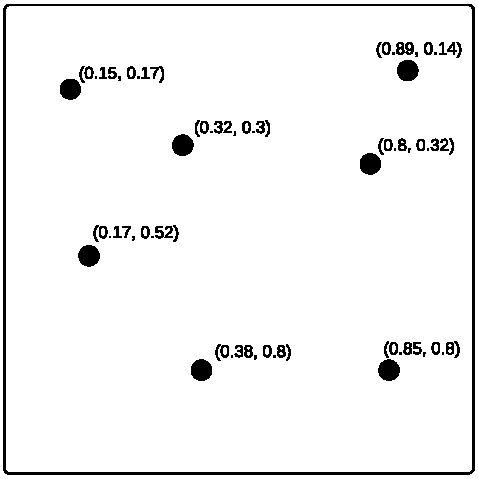
\includegraphics[scale=0.6]{figures/2D_data_space.pdf}
	\end{center}
	\vspace{-40pt}
	\caption{Data items represented as 2D points in the space $[0, 1]^d$ (not to scale)}
	\label{fig:data-space}
\end{wrapfigure}

The purpose of an index structure is to perform queries on the data. Common types of query include:
\begin{itemize}
	\item \textbf{Point Query} -- checks if a point $p$ exists in the structure \cite{rplus-tree}
	\item \textbf{Region/Range Query} -- return all points contained within a spatial region $r$ \cite{rplus-tree}, which is often a $d$-dimensional box \cite{r-tree, pk-tree, pyramid-tree}
	\item \textbf{\textit{k}-Nearest Neighbour Search} -- return the $k$ nearest points to a point $p$ \cite{pk-tree}
	\item \textbf{Approximate Nearest Neighbour Search} -- return an approximation of a $k$-nearest neighbour search \cite{knn-curse-of-dimensionality} (less accuracy, faster queries)
\end{itemize}

An index structure provides a mechanism for accessing multi-dimensional data, but it may not actually store the data itself. In a database for example, a point query comes in two parts: \textbf{searching} for a data point in the structure and \textbf{reading} the data from the data file represented by point (or index) \cite{rsr-tree}.
